\documentclass[a4paper,10pt, twocolumn]{report}
\usepackage[utf8]{inputenc}
\usepackage{graphicx}
\usepackage[font=footnotesize]{caption}
\usepackage{mathtools}

% Title Page
\title{Photodiode Amplifier Design for Optical Vibrometry}
\author{Joseph Mariglio}


\begin{document}
\maketitle

\begin{abstract}

\end{abstract}
The central goal of this project is to design a geometric optical vibrometer array. 
This device will be capable of measuring transverse waves across a wide band of frequencies, without mass-loading the object. 
The design parameters to be minimized include cost, power consumption, and noise floor. 
The parameters to be maximized include signal gain, bandwidth, and versatility. 
The device is intended to be suitable for both researchers and artists interested in mechanical vibrations.

To suit both minimizing and maximizing constraints, much of the precision will be offloaded from potentially expensive optical or mechanical components, onto the integrated processor and supporting electronics, which can be scaled much more cheaply. As a result, techniques such as interferometry will be eschewed in favor of simpler measurement regimes, which are more tolerant to error. Examples of mixed signal processing techniques which will be explored include differential current measurement, inverse filtering, and source multiplexing. An array of vibrometers affords the designer to use techniques such as dynamic modal analysis, cross-talk cancellation, and various image processing techniques to further digitally enhance the signal.

A geometric optical vibrometer measures the displacement of an object using the Law of Reflection\cite[p.~95]{<hecht87>}. This law, which holds true for incident ray bundles on an interface of appropriate smoothness to exhibit specular reflection, states that the angle-of-incidence equals the angle-of-reflection, i.e.: $\theta _{i} = \theta _{r}$ . The device uses a light source and a light sensor, at points $a$ and $b$, respectively. These points $a$ and $b$ lie on a line approximately parallel to the region of the surface being measured, which is at a distance of $x$ from $ab$. The light source is aimed at an angle $\theta _i$  subtended from the normal, so that the emitted rays reflect off of the surface at $a$ point $c$, at the same angle $\theta _{r}$, to be projected back onto the light sensor at some new location $d$. The plane spanned by $a b c$ is called the “plane-of-incidence.” This plane should be perpendicular to the plane of the surface being measured, or else $d$ will not be coplanar. \cite{
<barb09>}
\begin{figure}[h]
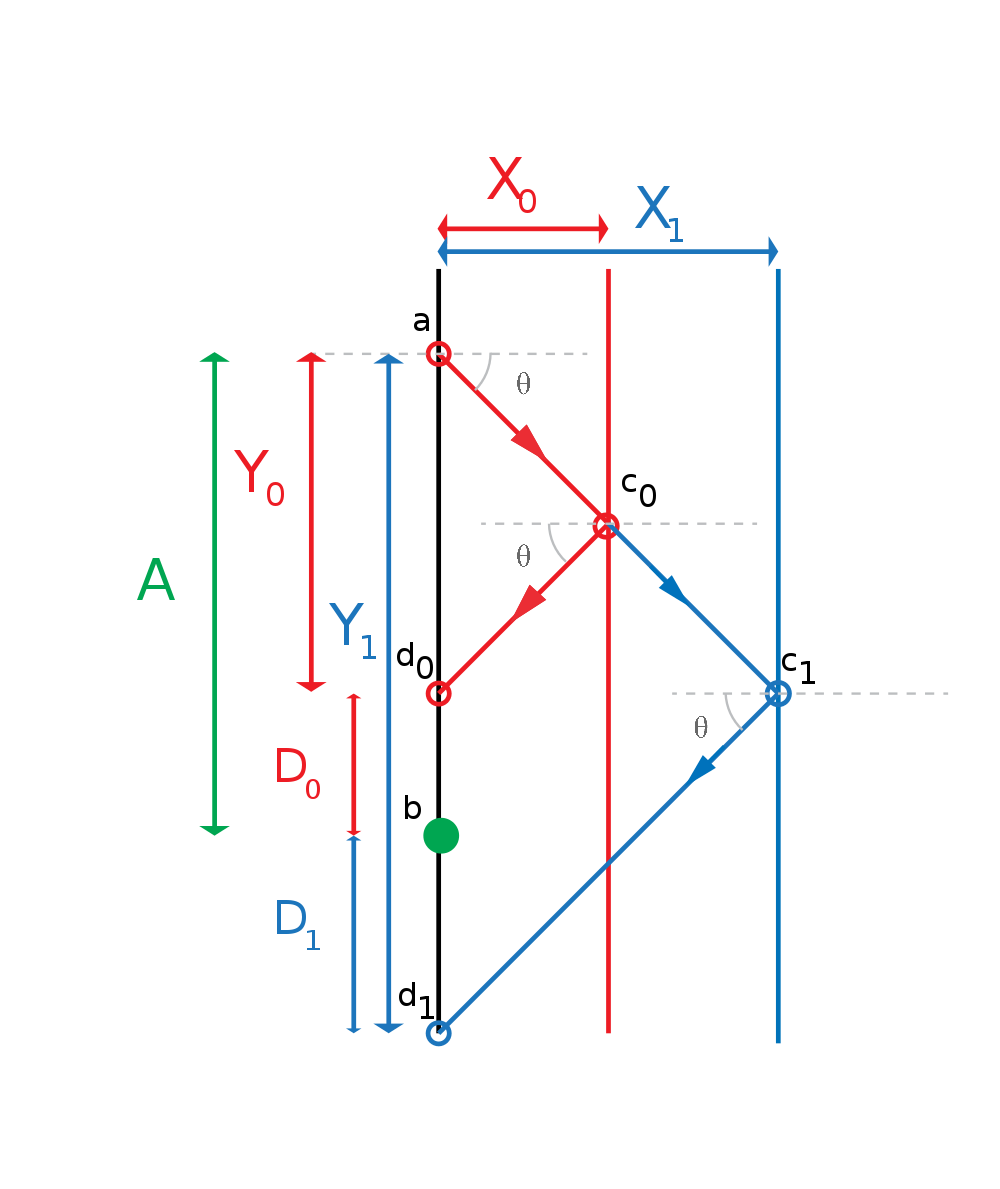
\includegraphics[scale=0.25]{./figures/displacement_measurement_points}
\caption{Light emitted from the point $a$ is projected onto the line $ab$ at locations $d0$ and $d1$ when the medium is at a distance of $X_0$ and $X_1$, respectively, which are proportional to distances $D_0$ and $D_1$.}
\end{figure}
Given that the sensor at $b$ can determine the radial distance of the incident rays by sensing optical power, the length of line segment ad can be calculated by adding the known length of line segment $ab$. The value of distance $X$ can then be calculated by considering the isoceles triangle $acd$, i.e.: $X = \frac{A + d}{2\tan\theta}$ However, this calculation does not preserve the sign of distance $D$, and therefore is only valid if the point $d$ never crosses $b$. Adding a second sensor on the line $ab$ and comparing measured optical power would solve this problem, but as of this time the author has found it sufficient to calibrate the system such that $d$ never crosses $b$.

Further limitations to this system require the distance $X$ to be relatively small. As $X$ becomes larger, the angular deviations in the medium are amplified. This will cause the returning ray bundle's angle-of-incidence to increase by the angle of surface deviation, i.e.: $\theta_r = \theta_i + \theta_d$. Finally, this equation is only true so long as the wavelength of surface features $\lambda_{surface}$ remain larger than the wavelength $\lambda_{light}$. As  $\lambda_{surface}$ nears $\lambda_{light}$, diffraction effects take over, and components of the reflection will not be totally specular. As a result, optical power in whatever reflected ray bundle remains incident on the sensor will be attenuated as increasingly more optical power is diffused. \cite[p.~96]{<hecht87>}

Finally, the sensor at $b$ measures the radial distance of an incident ray bundle as a linear function of radiant flux density, $\phi_e$  because of diffraction effects on the edges of the ray bundle, which are caused by the aperture through which the bundle was emitted. These fringe patterns are spatially averaged across the surface of the sensor, yielding a smooth, nearly linear response curve. This curve could be made more linear by adding a second aperture, tapered to one side, at the sensor. The author has not found this additional constraint necessary at this time. 

A typical high-bandwidth light-sensing component is the photodiode. All semiconductors react to incident photons, but a photodiode has been constructed specifically to interact with certain bandwidths of light in a known way. A diode consists of a positively “p” doped and negatively “n” doped semiconductor junction, with a nearly neutral or “intrinsic” layer separating them. Photodiodes react to incident photons by creating electon-hole pairs, which carry a charge to the “n” and “p” terminals, respectively. For a given photon, this process can occur according to one of two time constants, “drift” or “diffusion”, depending on where the incident photon meets the component. Since many photons are typically incident on a photodiode during its operation, these two time constants are observed simultaneously, and add to each other. When a photon is incident on an intrinsic semiconductor, the electron-hole pairs are transported quickly to their respective terminals, unimpeded by the charge bias of either the “p” or “
n” doped materials. However, when a photon is incident on either the “p” or “n” doped terminals, an electron-hole pair travels by diffusion, and could either survive the trip to the “i” region or recombine and cancel. This process is much slower than drift.\cite[p.~3]{<graeme96>} As a result, “PIN” photodiodes are manufactured with a larger intrinsic region to take advantage of this effect. Reverse biasing can also increase the intrinsic region and improve bandwidth, at the cost of current leakage.	

A photodiode can operate in one of two modes: “photoconductive” or “photovoltaic.” In photoconductive mode, the voltage across the photodiode ep is held at a value $\leq 0$. In this case, the current passing through the photodiode it is only affected by the current response to incident photons $i_p$. This relationship is linear but inverted. Bandwidth increases as $e_p$ grows more negative. By contrast, in photovoltaic mode, the diode generates a voltage in response to incident photons. The diode is being forward biased, which causes a reduction in bandwidth by shrinking the intrinsic layer. The current passing through the diode is influenced by both the current passing through the diode $i_d$ and the current response to incident photons $i_p$. Furthermore, $e_p$ bears a logarithmic relationship to $i_p$ in photovoltaic mode. Generally speaking, photovoltaic measurements trade bandwidth for sensitivity.\cite[p.~7]{<graeme96>}

The author's device uses a PIN photodiode in zero-biased photoconductive mode, which offered the best compromise between bandwidth and leakage current. To read the current-encoded optical power signal, it must first be converted into a voltage. A transimpedance amplifier does exactly this.\cite[p.~561]{<scherz07>} The TIA is the essential building-block for most high-bandwidth photodiode amplifiers.\cite[p.~30]{<graeme96>} 

Most of the development time so far has been spent on the transimpedance amplifier of the device. The goal has been to maximize parameters such as gain, bandwidth, SNR, and EMI rejection, while minimizing phase distortion, THD, current draw, and cost. At this time, there have been eight major revisions to the topology of the pickup amplifier alone. Methods for assessing components of the system, primarily the photodiode amplifier and laser emitter driver circuits, have been developed which employ a variation on the linearly swept sine (“linear chirp”) technique for time-invariant systems.\cite{<farina07>} STFT-based spectrograms and time-domain SNR measurements have also contributed to a hybrid testing approach, with the intention of assessing many parameters with each test.

In testing the TIA, the author started by attempting to recreate the field conditions under which this device should operate. The author naively set out to measure vibrations on a mirror, reflecting the light from a stationary laser diode off of a mirror and onto a stationary photodiode. The mirror was coupled to an electromechanical transducer, which turned voltage-encoded signals into mechanical vibrations. As a control, a piezoelectric pickup was coupled to the mirror in an attempt to measure the mirror's response to vibrations. A direct recording of the digital test signals was used as a control. The photodiode's current was picked up by a series of amplifier circuits, which were the object of inquiry. 

Chirps were sent through system via the vibrational transducer across the entire sampled spectrum (0-96kHz). Since this was such an early stage of development, the analysis tools largely revolved around STFT spectrograms. However, for the last two circuits tested with this experimental setup, transfer functions were directly calculated via acyclic deconvolution.\cite{<farina07>} Later circuits were also tested with a sinusoidally modulated light-source, which were demodulated after digitization. 

The circuits tested under these conditions, named “a” - “f,” each showed improvement over their predecessors, but still were unacceptable for one reason or another. For example, the “e” family incorporated a two-pole highpass filter into the current amplifier, in an attempt to duck the interference measured at 60hz and multiples thereof. While this technique was successful at removing this low frequency EMI and DC offset, the phase response was non-linear, and the frequency response was markedly uneven. While integrating the highpass filter into the TIA improved the bandwidth, the circuit became much more difficult to analyze. Furthermore, the “e” family of amplifiers seemed to exhibit strange behavior after modulating and demodulating. Although the broadband (unmodulated) signal sounded free of noise, there were in fact bands of interference in several regions above 40kHz and above 90kHz. Upon demodulation, these frequencies would be shifted down into the audible spectrum, along with the signal. As a result 
of these findings, the author omitted the highpass filter from the design. The last amplifier of this test series-- the “f” family-- had a SNR of 18.2 dB in the dark, and 3.5 dB with fluorescent lights on. These amplifiers were clearly not useful for any sort of precision measurement.

\bibliographystyle{plain}
\bibliography{photodiode_paper.bib}
\end{document}
